\documentclass[12pt]{article}

%packages
%\usepackage{latexsym}
\usepackage{graphicx}
\usepackage{color}
\usepackage{amsmath}
\usepackage{dsfont}
\usepackage{placeins}
\usepackage{amssymb}
\usepackage{wasysym}
\usepackage{abstract}
\usepackage{hyperref}
\usepackage{etoolbox}
\usepackage{datetime}
\usepackage{xcolor}
\usepackage{alphalph}
\usepackage{bm}
\settimeformat{ampmtime}

%\usepackage{pstricks,pst-node,pst-tree}

%\usepackage{algpseudocode}
%\usepackage{amsthm}
%\usepackage{hyperref}
%\usepackage{mathrsfs}
%\usepackage{amsfonts}
%\usepackage{bbding}
%\usepackage{listings}
%\usepackage{appendix}
\usepackage[margin=1in]{geometry}
%\geometry{papersize={8.5in,11in},total={6.5in,9in}}
%\usepackage{cancel}
%\usepackage{algorithmic, algorithm}

\makeatletter
\def\maxwidth{ %
  \ifdim\Gin@nat@width>\linewidth
    \linewidth
  \else
    \Gin@nat@width
  \fi
}
\makeatother

\definecolor{fgcolor}{rgb}{0.345, 0.345, 0.345}
\newcommand{\hlnum}[1]{\textcolor[rgb]{0.686,0.059,0.569}{#1}}%
\newcommand{\hlstr}[1]{\textcolor[rgb]{0.192,0.494,0.8}{#1}}%
\newcommand{\hlcom}[1]{\textcolor[rgb]{0.678,0.584,0.686}{\textit{#1}}}%
\newcommand{\hlopt}[1]{\textcolor[rgb]{0,0,0}{#1}}%
\newcommand{\hlstd}[1]{\textcolor[rgb]{0.345,0.345,0.345}{#1}}%
\newcommand{\hlkwa}[1]{\textcolor[rgb]{0.161,0.373,0.58}{\textbf{#1}}}%
\newcommand{\hlkwb}[1]{\textcolor[rgb]{0.69,0.353,0.396}{#1}}%
\newcommand{\hlkwc}[1]{\textcolor[rgb]{0.333,0.667,0.333}{#1}}%
\newcommand{\hlkwd}[1]{\textcolor[rgb]{0.737,0.353,0.396}{\textbf{#1}}}%

\usepackage{framed}
\makeatletter
\newenvironment{kframe}{%
 \def\at@end@of@kframe{}%
 \ifinner\ifhmode%
  \def\at@end@of@kframe{\end{minipage}}%
  \begin{minipage}{\columnwidth}%
 \fi\fi%
 \def\FrameCommand##1{\hskip\@totalleftmargin \hskip-\fboxsep
 \colorbox{shadecolor}{##1}\hskip-\fboxsep
     % There is no \\@totalrightmargin, so:
     \hskip-\linewidth \hskip-\@totalleftmargin \hskip\columnwidth}%
 \MakeFramed {\advance\hsize-\width
   \@totalleftmargin\z@ \linewidth\hsize
   \@setminipage}}%
 {\par\unskip\endMakeFramed%
 \at@end@of@kframe}
\makeatother

\definecolor{shadecolor}{rgb}{.77, .77, .77}
\definecolor{messagecolor}{rgb}{0, 0, 0}
\definecolor{warningcolor}{rgb}{1, 0, 1}
\definecolor{errorcolor}{rgb}{1, 0, 0}
\newenvironment{knitrout}{}{} % an empty environment to be redefined in TeX

\usepackage{alltt}
\usepackage[T1]{fontenc}

\newcommand{\qu}[1]{``#1''}
\newcounter{probnum}
\setcounter{probnum}{1}

%create definition to allow local margin changes
\def\changemargin#1#2{\list{}{\rightmargin#2\leftmargin#1}\item[]}
\let\endchangemargin=\endlist 

%allow equations to span multiple pages
\allowdisplaybreaks

%define colors and color typesetting conveniences
\definecolor{gray}{rgb}{0.5,0.5,0.5}
\definecolor{black}{rgb}{0,0,0}
\definecolor{white}{rgb}{1,1,1}
\definecolor{blue}{rgb}{0.5,0.5,1}
\newcommand{\inblue}[1]{\color{blue}#1 \color{black}}
\definecolor{green}{rgb}{0.133,0.545,0.133}
\newcommand{\ingreen}[1]{\color{green}#1 \color{black}}
\definecolor{yellow}{rgb}{1,1,0}
\newcommand{\inyellow}[1]{\color{yellow}#1 \color{black}}
\definecolor{orange}{rgb}{0.9,0.649,0}
\newcommand{\inorange}[1]{\color{orange}#1 \color{black}}
\definecolor{red}{rgb}{1,0.133,0.133}
\newcommand{\inred}[1]{\color{red}#1 \color{black}}
\definecolor{purple}{rgb}{0.58,0,0.827}
\newcommand{\inpurple}[1]{\color{purple}#1 \color{black}}
\definecolor{backgcode}{rgb}{0.97,0.97,0.8}
\definecolor{Brown}{cmyk}{0,0.81,1,0.60}
\definecolor{OliveGreen}{cmyk}{0.64,0,0.95,0.40}
\definecolor{CadetBlue}{cmyk}{0.62,0.57,0.23,0}

%define new math operators
\DeclareMathOperator*{\argmax}{arg\,max~}
\DeclareMathOperator*{\argmin}{arg\,min~}
\DeclareMathOperator*{\argsup}{arg\,sup~}
\DeclareMathOperator*{\arginf}{arg\,inf~}
\DeclareMathOperator*{\convolution}{\text{\Huge{$\ast$}}}
\newcommand{\infconv}[2]{\convolution^\infty_{#1 = 1} #2}
%true functions

%%%% GENERAL SHORTCUTS

%shortcuts for pure typesetting conveniences
\newcommand{\bv}[1]{\boldsymbol{#1}}

%shortcuts for compound constants
\newcommand{\BetaDistrConst}{\dfrac{\Gamma(\alpha + \beta)}{\Gamma(\alpha)\Gamma(\beta)}}
\newcommand{\NormDistrConst}{\dfrac{1}{\sqrt{2\pi\sigma^2}}}

%shortcuts for conventional symbols
\newcommand{\tsq}{\tau^2}
\newcommand{\tsqh}{\hat{\tau}^2}
\newcommand{\sigsq}{\sigma^2}
\newcommand{\sigsqsq}{\parens{\sigma^2}^2}
\newcommand{\sigsqovern}{\dfrac{\sigsq}{n}}
\newcommand{\tausq}{\tau^2}
\newcommand{\tausqalpha}{\tau^2_\alpha}
\newcommand{\tausqbeta}{\tau^2_\beta}
\newcommand{\tausqsigma}{\tau^2_\sigma}
\newcommand{\betasq}{\beta^2}
\newcommand{\sigsqvec}{\bv{\sigma}^2}
\newcommand{\sigsqhat}{\hat{\sigma}^2}
\newcommand{\sigsqhatmlebayes}{\sigsqhat_{\text{Bayes, MLE}}}
\newcommand{\sigsqhatmle}[1]{\sigsqhat_{#1, \text{MLE}}}
\newcommand{\bSigma}{\bv{\Sigma}}
\newcommand{\bSigmainv}{\bSigma^{-1}}
\newcommand{\thetavec}{\bv{\theta}}
\newcommand{\thetahat}{\hat{\theta}}
\newcommand{\thetahatmle}{\hat{\theta}_{\mathrm{MLE}}}
\newcommand{\thetavechatmle}{\hat{\thetavec}_{\mathrm{MLE}}}
\newcommand{\muhat}{\hat{\mu}}
\newcommand{\musq}{\mu^2}
\newcommand{\muvec}{\bv{\mu}}
\newcommand{\muhatmle}{\muhat_{\text{MLE}}}
\newcommand{\lambdahat}{\hat{\lambda}}
\newcommand{\lambdahatmle}{\lambdahat_{\text{MLE}}}
\newcommand{\etavec}{\bv{\eta}}
\newcommand{\alphavec}{\bv{\alpha}}
\newcommand{\minimaxdec}{\delta^*_{\mathrm{mm}}}
\newcommand{\ybar}{\bar{y}}
\newcommand{\xbar}{\bar{x}}
\newcommand{\Xbar}{\bar{X}}
\newcommand{\phat}{\hat{p}}
\newcommand{\Phat}{\hat{P}}
\newcommand{\Zbar}{\bar{Z}}
\newcommand{\iid}{~{\buildrel iid \over \sim}~}
\newcommand{\inddist}{~{\buildrel ind \over \sim}~}
\newcommand{\approxdist}{~{\buildrel approx \over \sim}~}
\newcommand{\equalsindist}{~{\buildrel d \over =}~}
\newcommand{\loglik}[1]{\ell\parens{#1}}
\newcommand{\thetahatkminone}{\thetahat^{(k-1)}}
\newcommand{\thetahatkplusone}{\thetahat^{(k+1)}}
\newcommand{\thetahatk}{\thetahat^{(k)}}
\newcommand{\half}{\frac{1}{2}}
\newcommand{\third}{\frac{1}{3}}
\newcommand{\twothirds}{\frac{2}{3}}
\newcommand{\fourth}{\frac{1}{4}}
\newcommand{\fifth}{\frac{1}{5}}
\newcommand{\sixth}{\frac{1}{6}}

%shortcuts for vector and matrix notation
\newcommand{\A}{\bv{A}}
\newcommand{\At}{\A^T}
\newcommand{\Ainv}{\inverse{\A}}
\newcommand{\B}{\bv{B}}
\newcommand{\K}{\bv{K}}
\newcommand{\Kt}{\K^T}
\newcommand{\Kinv}{\inverse{K}}
\newcommand{\Kinvt}{(\Kinv)^T}
\newcommand{\M}{\bv{M}}
\newcommand{\Bt}{\B^T}
\newcommand{\Q}{\bv{Q}}
\newcommand{\Qt}{\Q^T}
\newcommand{\R}{\bv{R}}
\newcommand{\Rt}{\R^T}
\newcommand{\Z}{\bv{Z}}
\newcommand{\X}{\bv{X}}
\renewcommand{\H}{\bv{H}}
\newcommand{\Xsub}{\X_{\text{(sub)}}}
\newcommand{\Xsubadj}{\X_{\text{(sub,adj)}}}
\newcommand{\I}{\bv{I}}
\newcommand{\Y}{\bv{Y}}
\newcommand{\sigsqI}{\sigsq\I}
\renewcommand{\P}{\bv{P}}
\newcommand{\Psub}{\P_{\text{(sub)}}}
\newcommand{\Pt}{\P^T}
\newcommand{\Pii}{P_{ii}}
\newcommand{\Pij}{P_{ij}}
\newcommand{\IminP}{(\I-\P)}
\newcommand{\Xt}{\bv{X}^T}
\newcommand{\XtX}{\Xt\X}
\newcommand{\XtXinv}{\parens{\Xt\X}^{-1}}
\newcommand{\XtXinvXt}{\XtXinv\Xt}
\newcommand{\XXtXinvXt}{\X\XtXinvXt}
\newcommand{\x}{\bv{x}}
\renewcommand{\b}{\bv{b}}
\newcommand{\onevec}{\bv{1}}
\newcommand{\oneton}{1, \ldots, n}
\newcommand{\yoneton}{y_1, \ldots, y_n}
\newcommand{\yonetonorder}{y_{(1)}, \ldots, y_{(n)}}
\newcommand{\Yoneton}{Y_1, \ldots, Y_n}
\newcommand{\iinoneton}{i \in \braces{\oneton}}
\newcommand{\onetom}{1, \ldots, m}
\newcommand{\jinonetom}{j \in \braces{\onetom}}
\newcommand{\xoneton}{x_1, \ldots, x_n}
\newcommand{\Xoneton}{X_1, \ldots, X_n}
\newcommand{\xt}{\x^T}
\newcommand{\y}{\bv{y}}
\newcommand{\yt}{\y^T}
\renewcommand{\c}{\bv{c}}
\newcommand{\ct}{\c^T}
\newcommand{\tstar}{\bv{t}^*}
\renewcommand{\u}{\bv{u}}
\renewcommand{\v}{\bv{v}}
\renewcommand{\a}{\bv{a}}
\newcommand{\s}{\bv{s}}
\newcommand{\yadj}{\y_{\text{(adj)}}}
\newcommand{\xjadj}{\x_{j\text{(adj)}}}
\newcommand{\xjadjM}{\x_{j \perp M}}
\newcommand{\yhat}{\hat{\y}}
\newcommand{\yhatsub}{\yhat_{\text{(sub)}}}
\newcommand{\yhatstar}{\yhat^*}
\newcommand{\yhatstarnew}{\yhatstar_{\text{new}}}
\newcommand{\z}{\bv{z}}
\newcommand{\zt}{\z^T}
\newcommand{\bb}{\bv{b}}
\newcommand{\bbt}{\bb^T}
\newcommand{\bbeta}{\bv{\beta}}
\newcommand{\beps}{\bv{\epsilon}}
\newcommand{\bepst}{\beps^T}
\newcommand{\e}{\bv{e}}
\newcommand{\Mofy}{\M(\y)}
\newcommand{\KofAlpha}{K(\alpha)}
\newcommand{\ellset}{\mathcal{L}}
\newcommand{\oneminalph}{1-\alpha}
\newcommand{\SSE}{\text{SSE}}
\newcommand{\SSEsub}{\text{SSE}_{\text{(sub)}}}
\newcommand{\MSE}{\text{MSE}}
\newcommand{\RMSE}{\text{RMSE}}
\newcommand{\SSR}{\text{SSR}}
\newcommand{\SST}{\text{SST}}
\newcommand{\JSest}{\delta_{\text{JS}}(\x)}
\newcommand{\Bayesest}{\delta_{\text{Bayes}}(\x)}
\newcommand{\EmpBayesest}{\delta_{\text{EmpBayes}}(\x)}
\newcommand{\BLUPest}{\delta_{\text{BLUP}}}
\newcommand{\MLEest}[1]{\hat{#1}_{\text{MLE}}}

%shortcuts for Linear Algebra stuff (i.e. vectors and matrices)
\newcommand{\twovec}[2]{\bracks{\begin{array}{c} #1 \\ #2 \end{array}}}
\newcommand{\threevec}[3]{\bracks{\begin{array}{c} #1 \\ #2 \\ #3 \end{array}}}
\newcommand{\fivevec}[5]{\bracks{\begin{array}{c} #1 \\ #2 \\ #3 \\ #4 \\ #5 \end{array}}}
\newcommand{\twobytwomat}[4]{\bracks{\begin{array}{cc} #1 & #2 \\ #3 & #4 \end{array}}}
\newcommand{\threebytwomat}[6]{\bracks{\begin{array}{cc} #1 & #2 \\ #3 & #4 \\ #5 & #6 \end{array}}}

%shortcuts for conventional compound symbols
\newcommand{\thetainthetas}{\theta \in \Theta}
\newcommand{\reals}{\mathbb{R}}
\newcommand{\complexes}{\mathbb{C}}
\newcommand{\rationals}{\mathbb{Q}}
\newcommand{\integers}{\mathbb{Z}}
\newcommand{\naturals}{\mathbb{N}}
\newcommand{\forallninN}{~~\forall n \in \naturals}
\newcommand{\forallxinN}[1]{~~\forall #1 \in \reals}
\newcommand{\matrixdims}[2]{\in \reals^{\,#1 \times #2}}
\newcommand{\inRn}[1]{\in \reals^{\,#1}}
\newcommand{\mathimplies}{\quad\Rightarrow\quad}
\newcommand{\mathlogicequiv}{\quad\Leftrightarrow\quad}
\newcommand{\eqncomment}[1]{\quad \text{(#1)}}
\newcommand{\limitn}{\lim_{n \rightarrow \infty}}
\newcommand{\limitN}{\lim_{N \rightarrow \infty}}
\newcommand{\limitd}{\lim_{d \rightarrow \infty}}
\newcommand{\limitt}{\lim_{t \rightarrow \infty}}
\newcommand{\limitsupn}{\limsup_{n \rightarrow \infty}~}
\newcommand{\limitinfn}{\liminf_{n \rightarrow \infty}~}
\newcommand{\limitk}{\lim_{k \rightarrow \infty}}
\newcommand{\limsupn}{\limsup_{n \rightarrow \infty}}
\newcommand{\limsupk}{\limsup_{k \rightarrow \infty}}
\newcommand{\floor}[1]{\left\lfloor #1 \right\rfloor}
\newcommand{\ceil}[1]{\left\lceil #1 \right\rceil}

%shortcuts for environments
\newcommand{\beqn}{\vspace{-0.25cm}\begin{eqnarray*}}
\newcommand{\eeqn}{\end{eqnarray*}}
\newcommand{\bneqn}{\vspace{-0.25cm}\begin{eqnarray}}
\newcommand{\eneqn}{\end{eqnarray}}

%shortcuts for mini environments
\newcommand{\parens}[1]{\left(#1\right)}
\newcommand{\squared}[1]{\parens{#1}^2}
\newcommand{\tothepow}[2]{\parens{#1}^{#2}}
\newcommand{\prob}[1]{\mathbb{P}\parens{#1}}
\newcommand{\cprob}[2]{\prob{#1~|~#2}}
\newcommand{\littleo}[1]{o\parens{#1}}
\newcommand{\bigo}[1]{O\parens{#1}}
\newcommand{\Lp}[1]{\mathbb{L}^{#1}}
\renewcommand{\arcsin}[1]{\text{arcsin}\parens{#1}}
\newcommand{\prodonen}[2]{\bracks{\prod_{#1=1}^n #2}}
\newcommand{\mysum}[4]{\sum_{#1=#2}^{#3} #4}
\newcommand{\sumonen}[2]{\sum_{#1=1}^n #2}
\newcommand{\infsum}[2]{\sum_{#1=1}^\infty #2}
\newcommand{\infprod}[2]{\prod_{#1=1}^\infty #2}
\newcommand{\infunion}[2]{\bigcup_{#1=1}^\infty #2}
\newcommand{\infinter}[2]{\bigcap_{#1=1}^\infty #2}
\newcommand{\infintegral}[2]{\int^\infty_{-\infty} #2 ~\text{d}#1}
\newcommand{\supthetas}[1]{\sup_{\thetainthetas}\braces{#1}}
\newcommand{\bracks}[1]{\left[#1\right]}
\newcommand{\braces}[1]{\left\{#1\right\}}
\newcommand{\set}[1]{\left\{#1\right\}}
\newcommand{\abss}[1]{\left|#1\right|}
\newcommand{\norm}[1]{\left|\left|#1\right|\right|}
\newcommand{\normsq}[1]{\norm{#1}^2}
\newcommand{\inverse}[1]{\parens{#1}^{-1}}
\newcommand{\rowof}[2]{\parens{#1}_{#2\cdot}}

%shortcuts for functionals
\newcommand{\realcomp}[1]{\text{Re}\bracks{#1}}
\newcommand{\imagcomp}[1]{\text{Im}\bracks{#1}}
\newcommand{\range}[1]{\text{range}\bracks{#1}}
\newcommand{\colsp}[1]{\text{colsp}\bracks{#1}}
\newcommand{\rowsp}[1]{\text{rowsp}\bracks{#1}}
\newcommand{\tr}[1]{\text{tr}\bracks{#1}}
\newcommand{\rank}[1]{\text{rank}\bracks{#1}}
\newcommand{\proj}[2]{\text{Proj}_{#1}\bracks{#2}}
\newcommand{\projcolspX}[1]{\text{Proj}_{\colsp{\X}}\bracks{#1}}
\newcommand{\median}[1]{\text{median}\bracks{#1}}
\newcommand{\mean}[1]{\text{mean}\bracks{#1}}
\newcommand{\dime}[1]{\text{dim}\bracks{#1}}
\renewcommand{\det}[1]{\text{det}\bracks{#1}}
\newcommand{\expe}[1]{\mathbb{E}\bracks{#1}}
\newcommand{\expeabs}[1]{\expe{\abss{#1}}}
\newcommand{\expesub}[2]{\mathbb{E}_{#1}\bracks{#2}}
\newcommand{\indic}[1]{\mathds{1}_{#1}}
\newcommand{\var}[1]{\mathbb{V}\text{ar}\bracks{#1}}
\newcommand{\cov}[2]{\mathbb{C}\text{ov}\bracks{#1, #2}}
\newcommand{\corr}[2]{\text{Corr}\bracks{#1, #2}}
\newcommand{\se}[1]{\mathbb{S}\text{E}\bracks{#1}}
\newcommand{\seest}[1]{\hat{\mathbb{S}\text{E}}\bracks{#1}}
\newcommand{\bias}[1]{\text{Bias}\bracks{#1}}
\newcommand{\derivop}[2]{\dfrac{\text{d}}{\text{d} #1}\bracks{#2}}
\newcommand{\partialop}[2]{\dfrac{\partial}{\partial #1}\bracks{#2}}
\newcommand{\secpartialop}[2]{\dfrac{\partial^2}{\partial #1^2}\bracks{#2}}
\newcommand{\mixpartialop}[3]{\dfrac{\partial^2}{\partial #1 \partial #2}\bracks{#3}}

%shortcuts for functions
\renewcommand{\exp}[1]{\mathrm{exp}\parens{#1}}
\renewcommand{\cos}[1]{\text{cos}\parens{#1}}
\renewcommand{\sin}[1]{\text{sin}\parens{#1}}
\newcommand{\sign}[1]{\text{sign}\parens{#1}}
\newcommand{\are}[1]{\mathrm{ARE}\parens{#1}}
\newcommand{\natlog}[1]{\ln\parens{#1}}
\newcommand{\oneover}[1]{\frac{1}{#1}}
\newcommand{\overtwo}[1]{\frac{#1}{2}}
\newcommand{\overn}[1]{\frac{#1}{n}}
\newcommand{\oneoversqrt}[1]{\oneover{\sqrt{#1}}}
\newcommand{\sqd}[1]{\parens{#1}^2}
\newcommand{\loss}[1]{\ell\parens{\theta, #1}}
\newcommand{\losstwo}[2]{\ell\parens{#1, #2}}
\newcommand{\cf}{\phi(t)}

%English language specific shortcuts
\newcommand{\ie}{\textit{i.e.} }
\newcommand{\AKA}{\textit{AKA} }
\renewcommand{\iff}{\textit{iff}}
\newcommand{\eg}{\textit{e.g.} }
\newcommand{\st}{\textit{s.t.} }
\newcommand{\wrt}{\textit{w.r.t.} }
\newcommand{\mathst}{~~\text{\st}~~}
\newcommand{\mathand}{~~\text{and}~~}
\newcommand{\ala}{\textit{a la} }
\newcommand{\ppp}{posterior predictive p-value}
\newcommand{\dd}{dataset-to-dataset}

%shortcuts for distribution titles
\newcommand{\logistic}[2]{\mathrm{Logistic}\parens{#1,\,#2}}
\newcommand{\bernoulli}[1]{\mathrm{Bernoulli}\parens{#1}}
\newcommand{\betanot}[2]{\mathrm{Beta}\parens{#1,\,#2}}
\newcommand{\stdbetanot}{\betanot{\alpha}{\beta}}
\newcommand{\multnormnot}[3]{\mathcal{N}_{#1}\parens{#2,\,#3}}
\newcommand{\normnot}[2]{\mathcal{N}\parens{#1,\,#2}}
\newcommand{\classicnormnot}{\normnot{\mu}{\sigsq}}
\newcommand{\stdnormnot}{\normnot{0}{1}}
\newcommand{\uniformdiscrete}[1]{\mathrm{Uniform}\parens{\braces{#1}}}
\newcommand{\uniform}[2]{\mathrm{U}\parens{#1,\,#2}}
\newcommand{\stduniform}{\uniform{0}{1}}
\newcommand{\geometric}[1]{\mathrm{Geometric}\parens{#1}}
\newcommand{\hypergeometric}[3]{\mathrm{Hypergeometric}\parens{#1,\,#2,\,#3}}
\newcommand{\exponential}[1]{\mathrm{Exp}\parens{#1}}
\newcommand{\gammadist}[2]{\mathrm{Gamma}\parens{#1, #2}}
\newcommand{\poisson}[1]{\mathrm{Poisson}\parens{#1}}
\newcommand{\binomial}[2]{\mathrm{Binomial}\parens{#1,\,#2}}
\newcommand{\negbin}[2]{\mathrm{NegBin}\parens{#1,\,#2}}
\newcommand{\rayleigh}[1]{\mathrm{Rayleigh}\parens{#1}}
\newcommand{\multinomial}[2]{\mathrm{Multinomial}\parens{#1,\,#2}}
\newcommand{\gammanot}[2]{\mathrm{Gamma}\parens{#1,\,#2}}
\newcommand{\cauchynot}[2]{\text{Cauchy}\parens{#1,\,#2}}
\newcommand{\invchisqnot}[1]{\text{Inv}\chisq{#1}}
\newcommand{\invscaledchisqnot}[2]{\text{ScaledInv}\ncchisq{#1}{#2}}
\newcommand{\invgammanot}[2]{\text{InvGamma}\parens{#1,\,#2}}
\newcommand{\chisq}[1]{\chi^2_{#1}}
\newcommand{\ncchisq}[2]{\chi^2_{#1}\parens{#2}}
\newcommand{\ncF}[3]{F_{#1,#2}\parens{#3}}

%shortcuts for PDF's of common distributions
\newcommand{\logisticpdf}[3]{\oneover{#3}\dfrac{\exp{-\dfrac{#1 - #2}{#3}}}{\parens{1+\exp{-\dfrac{#1 - #2}{#3}}}^2}}
\newcommand{\betapdf}[3]{\dfrac{\Gamma(#2 + #3)}{\Gamma(#2)\Gamma(#3)}#1^{#2-1} (1-#1)^{#3-1}}
\newcommand{\normpdf}[3]{\frac{1}{\sqrt{2\pi#3}}\exp{-\frac{1}{2#3}(#1 - #2)^2}}
\newcommand{\normpdfvarone}[2]{\dfrac{1}{\sqrt{2\pi}}e^{-\half(#1 - #2)^2}}
\newcommand{\chisqpdf}[2]{\dfrac{1}{2^{#2/2}\Gamma(#2/2)}\; {#1}^{#2/2-1} e^{-#1/2}}
\newcommand{\invchisqpdf}[2]{\dfrac{2^{-\overtwo{#1}}}{\Gamma(#2/2)}\,{#1}^{-\overtwo{#2}-1}  e^{-\oneover{2 #1}}}
\newcommand{\exponentialpdf}[2]{#2\exp{-#2#1}}
\newcommand{\poissonpdf}[2]{\dfrac{e^{-#1} #1^{#2}}{#2!}}
\newcommand{\binomialpdf}[3]{\binom{#2}{#1}#3^{#1}(1-#3)^{#2-#1}}
\newcommand{\rayleighpdf}[2]{\dfrac{#1}{#2^2}\exp{-\dfrac{#1^2}{2 #2^2}}}
\newcommand{\gammapdf}[3]{\dfrac{#3^#2}{\Gamma\parens{#2}}#1^{#2-1}\exp{-#3 #1}}
\newcommand{\cauchypdf}[3]{\oneover{\pi} \dfrac{#3}{\parens{#1-#2}^2 + #3^2}}
\newcommand{\Gammaf}[1]{\Gamma\parens{#1}}

%shortcuts for miscellaneous typesetting conveniences
\newcommand{\notesref}[1]{\marginpar{\color{gray}\tt #1\color{black}}}

%%%% DOMAIN-SPECIFIC SHORTCUTS

%Real analysis related shortcuts
\newcommand{\zeroonecl}{\bracks{0,1}}
\newcommand{\forallepsgrzero}{\forall \epsilon > 0~~}
\newcommand{\lessthaneps}{< \epsilon}
\newcommand{\fraccomp}[1]{\text{frac}\bracks{#1}}

%Bayesian related shortcuts
\newcommand{\yrep}{y^{\text{rep}}}
\newcommand{\yrepisq}{(\yrep_i)^2}
\newcommand{\yrepvec}{\bv{y}^{\text{rep}}}


%Probability shortcuts
\newcommand{\SigField}{\mathcal{F}}
\newcommand{\ProbMap}{\mathcal{P}}
\newcommand{\probtrinity}{\parens{\Omega, \SigField, \ProbMap}}
\newcommand{\convp}{~{\buildrel p \over \rightarrow}~}
\newcommand{\convLp}[1]{~{\buildrel \Lp{#1} \over \rightarrow}~}
\newcommand{\nconvp}{~{\buildrel p \over \nrightarrow}~}
\newcommand{\convae}{~{\buildrel a.e. \over \longrightarrow}~}
\newcommand{\convau}{~{\buildrel a.u. \over \longrightarrow}~}
\newcommand{\nconvau}{~{\buildrel a.u. \over \nrightarrow}~}
\newcommand{\nconvae}{~{\buildrel a.e. \over \nrightarrow}~}
\newcommand{\convd}{~{\buildrel \mathcal{D} \over \rightarrow}~}
\newcommand{\nconvd}{~{\buildrel \mathcal{D} \over \nrightarrow}~}
\newcommand{\withprob}{~~\text{w.p.}~~}
\newcommand{\io}{~~\text{i.o.}}

\newcommand{\Acl}{\bar{A}}
\newcommand{\ENcl}{\bar{E}_N}
\newcommand{\diam}[1]{\text{diam}\parens{#1}}

\newcommand{\taua}{\tau_a}

\newcommand{\myint}[4]{\int_{#2}^{#3} #4 \,\text{d}#1}
\newcommand{\laplacet}[1]{\mathscr{L}\bracks{#1}}
\newcommand{\laplaceinvt}[1]{\mathscr{L}^{-1}\bracks{#1}}
\renewcommand{\min}[1]{\text{min}\braces{#1}}
\renewcommand{\max}[1]{\text{max}\braces{#1}}

\newcommand{\Vbar}[1]{\bar{V}\parens{#1}}
\newcommand{\expnegrtau}{\exp{-r\tau}}

%%% problem typesetting
\definecolor{darkgrey}{rgb}{0.10,0.10,0.9}

\newcommand{\problem}[1]{\noindent \colorbox{black}{{\color{yellow} \large{\textsf{\textbf{Problem \arabic{probnum}}}}~}} \addtocounter{probnum}{1} \vspace{0.2cm} \\ \iftoggle{professormode}{}{\color{darkgrey}} #1}

\newcommand{\easysubproblem}[1]{\ingreen{\item} \iftoggle{professormode}{}{\color{darkgrey}} [easy] #1 \color{black} }
\newcommand{\intermediatesubproblem}[1]{\inorange{\item} \iftoggle{professormode}{}{\color{darkgrey}} [harder] #1 \color{black} }
\newcommand{\hardsubproblem}[1]{\inred{\item} \iftoggle{professormode}{}{\color{darkgrey}} [difficult] #1 \color{black} }
\newcommand{\extracreditsubproblem}[1]{\inpurple{\item} \iftoggle{professormode}{}{\color{darkgrey}} [E.C.] #1 \color{black} }


\newcommand{\spc}[1]{\iftoggle{professormode}{\\ \vspace{#1cm}}{\\ \vspace{-0.3cm}}}

\makeatletter
\newalphalph{\alphmult}[mult]{\@alph}{26}
\renewcommand{\labelenumi}{(\alphmult{\value{enumi}})}

\newcommand{\support}[1]{\text{Supp}\bracks{#1}}
\newcommand{\mode}[1]{\text{Mode}\bracks{#1}}
\newcommand{\IQR}[1]{\text{IQR}\bracks{#1}}
\newcommand{\quantile}[2]{\text{Quantile}\bracks{#1,\,#2}}


\newtoggle{professormode}
%\toggletrue{professormode} %STUDENTS: DELETE or COMMENT this line



\title{MATH 342W / 642 / RM742 Spring \the\year~HW \#1}

\author{Sergio E. Garcia Tapia} %STUDENTS: write your name here

\iftoggle{professormode}{
\date{Due 11:59PM February 5~on github\\ \vspace{0.5cm} \small (this document last updated \currenttime~on \today)}
}

\renewcommand{\abstractname}{Instructions and Philosophy}

\begin{document}
\maketitle

\iftoggle{professormode}{
\begin{abstract}
The path to success in this class is to do many problems. Unlike other courses, exclusively doing reading(s) will not help. Coming to lecture is akin to watching workout videos; thinking about and solving problems on your own is the actual ``working out.''  Feel free to \qu{work out} with others; \textbf{I want you to work on this in groups.}

Reading is still \textit{required}. For this homework set, read the first chapter of \qu{Learning from Data} and the introduction and Chapter 1 of Silver's book. Of course, you should be googling and reading about all the concepts introduced in class online. This is your responsibility to supplement in-class with your own readings.

The problems below are color coded: \ingreen{green} problems are considered \textit{easy} and marked \qu{[easy]}; \inorange{yellow} problems are considered \textit{intermediate} and marked \qu{[harder]}, \inred{red} problems are considered \textit{difficult} and marked \qu{[difficult]} and \inpurple{purple} problems are extra credit. The \textit{easy} problems are intended to be ``giveaways'' if you went to class. Do as much as you can of the others; I expect you to at least attempt the \textit{difficult} problems. 

This homework is worth 100 points but the point distribution will not be determined until after the due date. See syllabus for the policy on late homework.

Up to 7 points are given as a bonus if the homework is typed using \LaTeX. Links to instaling \LaTeX~and program for compiling \LaTeX~is found on the syllabus. You are encouraged to use \url{overleaf.com}. If you are handing in homework this way, read the comments in the code; there are two lines to comment out and you should replace my name with yours and write your section. The easiest way to use overleaf is to copy the raw text from hwxx.tex and preamble.tex into two new overleaf tex files with the same name. If you are asked to make drawings, you can take a picture of your handwritten drawing and insert them as figures or leave space using the \qu{$\backslash$vspace} command and draw them in after printing or attach them stapled.

The document is available with spaces for you to write your answers. If not using \LaTeX, print this document and write in your answers. I do not accept homeworks which are \textit{not} on this printout. Keep this first page printed for your records.

\end{abstract}

\thispagestyle{empty}
\vspace{1cm}
NAME: \line(1,0){380}
\clearpage
}

\problem{These are questions about Silver's book, the introduction and chapter 1.}

\begin{enumerate}

\easysubproblem{What is the difference between \emph{predict} and \emph{forecast}? Are these two terms used interchangably today?}\spc{4}

To forecast means to conjecture that something will occur based on previous
observations, information, or experience that a person may have. According to
Silver, on page 5, the terms are used interchangeably today. He mentions that
the term \emph{predict} had a more otherworldly meaning, such as a fortune
teller telling you that they see something in the future without necessarily
any evidence or scientific justification.

\easysubproblem{What is John P. Ioannidis's findings and what are its implications?}\spc{5}

On page 11, Silver shares that Ioannidis concluded it would not be possible to successfully
carry out many of the experiments that are posted in peer-reviewed journals related to
biomedical research. It implies that while the theoretical results in research may
be useful for modeling the world, we ought to be careful in the predictions that we make
based on them. If we misinterpret the data that we gather or make invalid assumptions
in our model, then this will turn affect the accuracy of our scientific predictions.

\easysubproblem{What are the human being's most powerful defense (according to Silver)? Answer using the language from class.}\spc{4}

According to Silver, it is the fact that we "simplify the world in ways that confirm our
biases". In other words, when we are awash with information, we make interpretations
that are convenient to us as if we wanted to validate a manufactured "truth", even if
the data says otherwise.

\easysubproblem{Information is increasing at a rapid pace, but what is not increasing?}\spc{3}

According to Silver, the amount of \emph{useful} information is not increasing, since
he argues that most of it is "noise". As a result, we have to spend a lot of energy
sifting through volumes of data, especially given that we retain much less than
we are awash with.

\hardsubproblem{Silver admits that we will always be subjectively biased when making predictions. However, he believes there is an objective truth. In class, how did we describe the objective truth? Answer using notation from class i.e. $t,f, g, h^*, \delta, \epsilon, t, z_1, \ldots, z_t, \delta, \mathbb{D}$, $\mathcal{H}, \mathcal{A}, \mathcal{X}, \mathcal{Y}, X, y, n, p$, $x_{\cdot 1}, \ldots, x_{\cdot p}, x_{1 \cdot}, \ldots, x_{n \cdot}$, etc.}\spc{3}

In class we talked about creating mathematical models as abstractions for reality.
In this context, the objective truth is represented by reality, such as the data
that we measure and that results from a system phenomenon in reality.
We assume that the universe is explained mathematically, so that a model
can be described by the functional relationship $y=t(z_1,\ldots,z_t)$ that remains
unknown to us. Our models of reality are based on observations captured by a set
$\mathbb{D}$ of input-output pairs of type $(x_k,y_k)$ such that $y_k=f(y_k)$, where
$x_1,\ldots,x_p$ are features that act as proxies for $z_1,\ldots,z_t$, and
$f$ is the best functional relationship we can get from the inputs.

\easysubproblem{In a nutshell, what is Karl Popper's (a famous philosopher of science) definition of \emph{science}?}\spc{4}

A discipline where hypotheses are falsifiable, in the sense that they can be "tested in the
real world by means of a prediction". In other words, it should be possible to design
an experiment and gather data that allows us to determine whether our assertions are
valid or not.

\intermediatesubproblem{Why did the ratings agencies say the probability of a CDO defaulting was 0.12\% instead of the 28\% that actually occurred? Answer using concepts from class.}\spc{4}

The ratings agencies assumed that the probability of their customers defaulting on their
CDO was largely independent. However, in reality they were largely correlated
as a result of housing prices rising.

\easysubproblem{What is the difference between \emph{risk} and \emph{uncertainty} according to Silver's definitions?}\spc{4}

Risk refers to a situation in which there is a nontrivial probability that it
will not result in a favorable outcome. Uncertainty is when we are aware of
the existence of risk, but we are unable to accurately quantify the probability
associated with said risk.

\hardsubproblem{How does Silver define \emph{out of sample}? Answer using notation from class i.e. $t,f, g, h^*, \delta, \epsilon, z_1, \ldots, z_t, \delta, \mathbb{D}, \mathcal{H}, \mathcal{A}, \mathcal{X}, \mathcal{Y}, X, y, n, p, x_{\cdot 1}, \ldots, x_{\cdot p}, x_{1 \cdot}, \ldots, x_{n \cdot}$, etc. WARNING: Silver defines \emph{out of sample} completely differently than the literature, than practitioners in industry and how we will define it in class in a month or so. We will explore what he is talking about in class in the future and we will term this concept differently, using the more widely accepted terminology. So please forget the phrase \emph{out of sample} for now as we will introduce it later in class as something else. There will be other such terms in his book and I will provide this disclaimer at these appropriate times.}\spc{7}

Silver uses out-of-sample to mean that we apply our previous experiences to a given
situation when in fact there are conditions that render our assumptions invalid.
Our approximation $g$ of the functional relationships $f$ and $t$ are computed using
the historical data $\mathbb{D}$ (e.g. driving sober). However, if we
then try to use $g$ on future data that does not result from the same phenomenon
(e.g. driving drunk), then the predictions from $g$ may not apply.

\intermediatesubproblem{Look up \emph{bias} and \emph{variance} online or in a statistics textbook. Connect these concepts to Silver's terms \emph{accuracy} and \emph{precision}. This is another example of Silver using non-standard terminology.}\spc{9}

By "precision", Silver means that data obtained from carrying out an experiment is consistent,
where values obtained are relatively close to one another (clustering together).
In "Introduction to Probability, Statistics, and Random Processes", Pishro-Nik,
explains that variance is a measure of how spread out the distribution of a random variable
is. Thus, higher precision as used by Silver corresponds to lower variance.

Silver thinks of high accuracy as obtaining a result in a model that closely behaves
like the phenomenon it is trying to describe in real life. In his book, Pishro-Nik
introduces the notion of bias in the context of estimators for quantities related to
a random variable. For example if we have a random variable $X$ for which we are
interested in the mean, an estimator is used to obtain a sample that has a distribution
that is identical to $X$ and the sample is used to estimate the mean. The bias of the
estimator is then used to describe how far on average it is from the real value.
In this case, the model is the estimator, and the real-life phenomenon is the real value
(for example, of the mean). A bias of $0$ corresponds to high accuracy as meant by Silver.

\end{enumerate}


\problem{Below are some questions about the theory of modeling.}

\begin{enumerate}

\easysubproblem{Redraw the illustration of Earth and the table-top globe except do not use the Earth and a table-top globe as examples (use another example). The quadrants are connected with arrows. Label these arrows appropriately.}\spc{11}

See Figure~\ref{fig:2a-flying}, where I have drawn the phenomenon of flying, and how airplanes
are modeled after birds doing this activity. I labeled the horizontal axes with possible
inputs such as the weight of the board, the drag force they experience, and so on,
and the output consists of their flying altitude and speed.

\begin{figure}
	\centering
	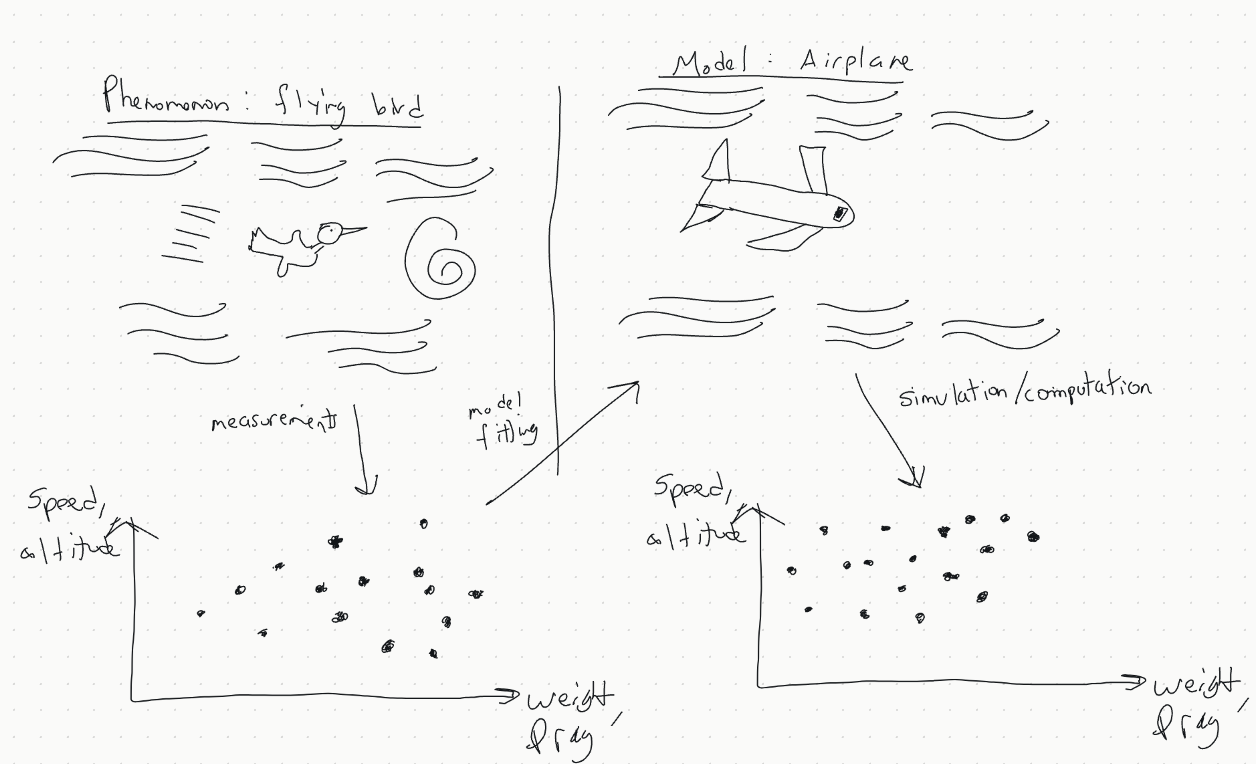
\includegraphics[width=0.7\textwidth]{exercise-2a-flying-phenomenon}
	\caption{Modeling the phenomenon of birds flying with airplanes.}
	\label{fig:2a-flying}
\end{figure}

\easysubproblem{Pursuant to the fix in the previous question, how do we define \emph{data} for the purposes of this class?}\spc{2}

Data refers to observations or measurements we make while observing a phenomenon manifest itself in real life.


\easysubproblem{Pursuant to the fix in the previous question, how do we define \emph{predictions} for the purposes of this class?}\spc{3}

Predictions are inferences that we make after experimenting with the data that we observe.
We obtain them from our model and they are meant to be approximations to real data.

\easysubproblem{Why are \qu{all models wrong}? We are quoting the famous statisticians George Box and Norman Draper here.}\spc{2}

Models attempt to capture essential characteristics of phenomena, but they make simplifying
assumptions in order to make it feasible to perform meaningful analysis. Whether knowingly or
unknowingly, they do not account for complex processes and interactions that are present
in the real-life phenomenon.

\intermediatesubproblem{Why are \qu{[some models] useful}? We are quoting the famous statisticians George Box and Norman Draper here.}\spc{2}

In spite of being wrong, models can provide insights that are still applicable. A model
does not need to exactly match the phenomenon that it is based on, as long as its provides
a close enough approximation for the purpose that one is trying to achieve. We use
models to try to make predictions, and though they are certainly wrong, they can still
be helpful for that.

\intermediatesubproblem{What is the difference between a "good model" and a "bad model"?}\spc{2}

One difference is the level of ambiguity. A good model results in positive validation,
where the predictions closely match the real-life data. A good model is also operational,
with inputs and outputs that are measurable, so that we can form falsifiable hypotheses.
A good model is unambiguous, with clear inputs and outputs, as well as the hypothesized
relationship that connects them.

\end{enumerate}




\problem{We are now going to investigate the famous English aphorism \qu{an apple a day keeps the doctor away} as a model. We will use this as springboard to ask more questions about the framework of modeling we introduced in this class.}

\begin{enumerate}


\easysubproblem{Is this a mathematical model? Yes / no and why.}\spc{3}

It is not a mathematical model because it is ambiguous. It appears to be a model for human health,
but the parameters that describe a person's health are not completely clear, nor are other aspects such as how many apples or the type of apple.

\easysubproblem{What is(are) the input(s) in this model?}\spc{3}

A given person, a given date, and whether the person ate apples on that date.

\easysubproblem{What is(are) the output(s) in this model?}\spc{3}

A given date and whether the person went to the doctor.

\intermediatesubproblem{How good / bad do you think this model is and why?}\spc{3}

It's not great because it supposes that apple consumption is strongly related to an
individual's health. Under this model, someone who does not eat apples at all
(perhaps because they dislike them) would need to visit the doctor often. It would
be more accurate if we instead identified and measured specific nutrient of apples and
the expected health benefit. The model also does not account for the specific reason why
someone is visiting the doctor. For example, a person might visit the doctor often
even though they eat a lot of apples, but their visit might be unrelated to their apple
consumption.

\easysubproblem{Devise a metric for gauging the main input. Call this $x_1$ going forward.}\spc{4}

The number of apples eaten since the age of 2.

\easysubproblem{Devise a metric for gauging the main output. Call this $y$ going forward.}\spc{4}

The number of visits to the doctor's office since the age of 2.

\easysubproblem{What is $\mathcal{Y}$ mathematically?}\spc{3}

$\mathcal{Y}=\mathbb{N}\cup \{0\}$, the set of natural numbers and $0$.

\easysubproblem{Briefly describe $z_1, \ldots, z_t$ in English where $y = t(z_1, \ldots, z_t)$ in this \emph{phenomenon} (not \emph{model}).}\spc{3}

The causal information $z_1,\ldots,z_t$ describes a person's health condition. It
consists of a person's medical history, symptoms they are showing, their diet, physical condition,
and more.

\easysubproblem{From this point on, you only observe $x_1$. What is the value of $p$?}\spc{1}

$p$ is the number of features. Since we only consider $x_1$, we have $p=1$.

\intermediatesubproblem{What is $\mathcal{X}$ mathematically? If your information contained in $x_1$ is non-numeric, you must coerce it to be numeric at this point.}\spc{3}

$\mathcal{X}=\mathbb{N}\cup\{0\}$, since it accounts for the number of apples a person
has eaten. It is the input space or covariate space.

\easysubproblem{How did we term the functional relationship between $y$ and $x_1$? Is it approximate or equals?}\spc{3}

In this class we are assuming that phenomena can be described mathematically. We said
that $y=f(x_1) + \delta$, where $\delta$ is the error due to ignorance, and $f$ is the
best functional relationship between the features and the response.

\easysubproblem{Briefly describe \emph{supervised learning}.}\spc{5}

Supervised learning is an approach to learning from data where we take examples observed as
a result of real-life phenomena, meaning that we have correct outputs corresponding to
certain inputs. The result is a rule that we use to predict real-life phenomena based on
inputs that do not come from the examples.

\easysubproblem{Why is \emph{supervised learning} an \emph{empirical solution} and not an \emph{analytic solution}?}\spc{3}

The empirical solution $g$ in supervised learning is obtained by considering the
behavior in a set of examples $\mathbb{D}$. The trouble is that we do not know
the behavior outside of $\mathbb{D}$, and there may be multiple analytic solutions
$f$ that agree with $g$ on $\mathbb{D}$. The supervised learning approach only tries
to predict behavior outside of $\mathbb{D}$, not match it exactly, so the solution
that it produces cannot be analytic.

\intermediatesubproblem{From this point on, assume we are involved in supervised learning to achieve the goal you stated in the previous question. Briefly describe what $\mathbb{D}$ would look like here.}\spc{3}

The set $\mathbb{D}$ is a collection of input-output pairs $(x_k,y_k)$, perhaps collected
by conducting a survey, where $x_k$ is the number of apples that a given person has eaten
since age $2$, and $y_k$ is the number of times that person has been to the doctor since age 2.

\intermediatesubproblem{Briefly describe the role of $\mathcal{H}$ and $\mathcal{A}$ here.}\spc{3}

$\mathcal{H}$ is the hypothesis set of functions $h$ that are thought to closely approximate
the behavior of the true analytic function $f$. The set encapsulates our assumptions about
the functional form we think describes $f$ appropriately. $\mathcal{A}$ is the learning algorithm
that we apply to arrive at an empirical solution $g$ from the hypothesis set $\mathcal{H}$ that best
approximates $f$ by using the examples $\mathbb{D}$ observed from the real-life phenomenon.

\easysubproblem{If $g = \mathcal{A}(\mathbb{D}, \mathcal{H})$, what should the domain and range of $g$ be?}\spc{3}

It should be the same domain as the functions in $\mathcal{H}$, and these in turn have the
same domain as the real-life phenomenon $f:\mathcal{X}\to\mathbb{Y}$. Hence the domain
is $\mathcal{X}$, the the range is $\mathcal{Y}$.

\easysubproblem{Is $g \in \mathcal{H}$? Why or why not?}\spc{3}

Yes. The set $\mathcal{H}$ has all of the hypothesis functions under considerations, those
that we believe may conceivably well-approximate $f$, and the algorithm $\mathcal{A}$
picks what it believes is the best one among them.

\easysubproblem{Given a never-before-seen value of $x_1$ which we denote $x^*$, what formula would we use to predict the corresponding value of the output? Denote this prediction $\hat{y}^*$.}\spc{1}

We would use $\hat{y}^* = g(x^*)$.

\intermediatesubproblem{$f$ is the function that is the best possible fit of the phenomenon given the covariates. We will unfortunately not be able to define \qu{best} until later in the course. But you can think of it as a device that extracts all possible information from the covariates and whatever is left over $\delta$ is due exclusively to information you do not have. Is it reasonable to assume $f \in \mathcal{H}$? Why or why not?}\spc{2}

No, it is not reasonable. We only know information about the function $f$ in $\mathbb{D}$,
and there are many functions, all with different properties, which may match $f$ at
such input-output pairs. It's possible that the assumptions we make lead to a hypothesis
set $\mathcal{H}$ that contains hypothesis functions that accurately approximate $f$ on
$\mathbb{D}$ but do not do well outside of $\mathbb{D}$.

\easysubproblem{In the general modeling setup, if $f \notin \mathcal{H}$, what are the three sources of error? Copy the equation from the class notes. Denote the names of each error and provide a sentence explanation of each. Denote also $e$ and $\mathcal{E}$ using underbraces / overbraces.}\spc{6}

In class we said that
\begin{align*}
	y &= t(z_1,\ldots,z_t)\\
	&=f(x_1,\ldots,x_p) + \delta\\
	&=h^*(x_1,\ldots,x_p) + \mathcal{E}\\
	&=g(x_1,\ldots,x_p)+e
\end{align*}

The three sources of errors are:
\begin{itemize}
	\item \emph{Ignorance error} $\delta= t-f$: It is the error incurred by the fact that
	our features $x_1,\ldots,x_p$ cannot possibly capture all the information implied by the
	true drivers $z_1,\ldots,z_t$.
	\item \emph{Misspecification error} $\mathcal{E}-\delta=f-h^*$: It is the error incurred
	by choosing a hypothesis set $\mathcal{H}$ that may not correctly capture the functional
	behavior of $f$. A more expansive $\mathcal{H}$ can lead to a decrease in this type of error.
	\item \emph{Estimation error} $h^*-g$: Error incurred by not having enough data examples
	in $\mathbb{D}$. We can decrease this by increasing the amount of data (i.e. increasing $n$).
\end{itemize}

\easysubproblem{In the general modeling setup, for each of the three source of error, explain what you would do to reduce the source of error as best as you can.}\spc{7}

\begin{itemize}
	\item \emph{Ignorance error}: Increase the number of relevant features (increase $p$).
	\item \emph{Misspecification error}: Choose a more expansive $\mathcal{H}$.
	\item \emph{Estimation error} $h^*-g$:  We can decrease this by increasing the amount of data (i.e. increasing $n$), or by improving the algorithm $\mathcal{A}$.
\end{itemize}

\intermediatesubproblem{In the general modeling setup, make up an $f$, an $h^*$ and a $g$ and plot them on a graph of $y$ vs $x$ (assume $p=1$). Indicate the sources of error on this plot (see last question). Which source of error is missing from the picture? Why?}\spc{9}

\begin{figure}
	\centering
	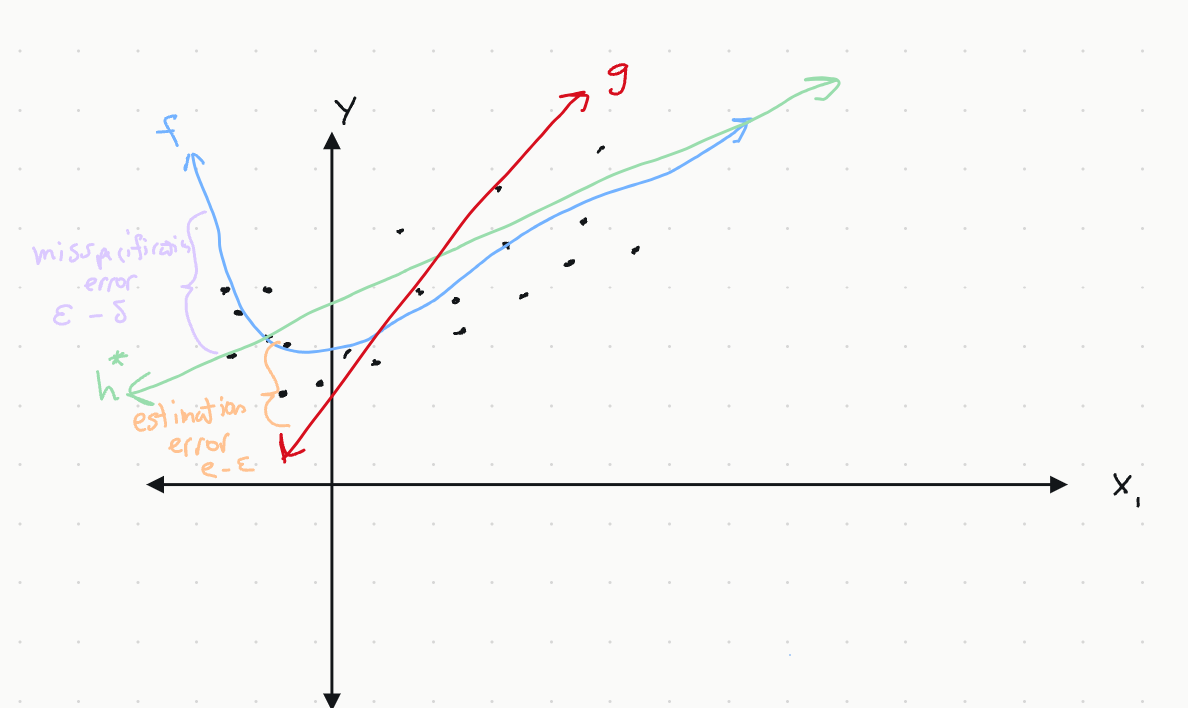
\includegraphics[width=0.7\textwidth]{3v-plot-f-h-g}
	\caption{Plot of $f$, $h^*$, and $g$ for a general model (Question 3v).}
	\label{fig:plot-3z}
\end{figure}
See Figure~\ref{fig:plot-3z}. The plot is missing $\delta$, the ignorance error. That error
is due to using insufficiently-many features to capture the information from the true
drivers. We cannot include them in the plot because aside from it not being possible
to know $t$ and the $z$'s, it would not be possible to plot them $t$ in the same
graph since it is a function of the $z$'s and not the features $x$'s.

\easysubproblem{What is a null model $g_0$? What data does it make use of? What data does it not make use of?}\spc{3}

A null model uses the mode statistic to determine the most common value. It is a constant
function whose output is that most repeated value. It makes use of the outputs $\vec{\mathbf{y}}$
from $\mathbb{D}$, and it does not make use of the inputs $\vec{\mathbf{x}}_i$ from $\mathbb{D}$.
The null model misclassifies any point whose output (response) does not equal the mode.
It serves a reference for performance of our algorithm. Since the null model does not take
any of the features into account, a good model that takes into account the features ought to have
a smaller misclassification error than the null model. Otherwise, either our algorithm is
poor, or our choice of features is poor.

\easysubproblem{What is a parameter in $\mathcal{H}$?}\spc{3}

It is a quantity that helps to identify a candidate function in $\mathcal{H}$, which
our algorithm tries to compute. For example, in the threshold model, the parameter
is a real number $\theta$ that determines the smallest value for which
our model would predict 1 as the response.

\easysubproblem{Regardless of your answer to what $\mathcal{Y}$ was above in (g), we now coerce $\mathcal{Y} = \braces{0,1}$. What would the null model $g_0$ be and why?}\spc{2}

The null model would be

\begin{align*}
	g_0 = \text{Mode}[\vec{\mathbf{y}}],\quad \vec{\mathbf{y}}\in \mathcal{Y}
\end{align*}

That is, it is a constant function whose value is either always $0$ or always $1$,
depending on which is more frequent among the values in our data set $\mathbb{D}$.

\easysubproblem{Regardless of your answer to what $\mathcal{Y}$ was above in (g), we now coerce $\mathcal{Y} = \braces{0,1}$. If we use a threshold model, what would $\mathcal{H}$ be? What would the parameter(s) be?}\spc{2}

We would have
\begin{align*}
	\mathcal{H}=\{\mathbb{I}_{x\geq \theta}: \theta\in\mathbb{N}\cup \{0\}\}
\end{align*}
Here, $\mathbb{I}$ is the indicator function. The parameter is $\theta$, the minimum number of apples
(the threshold) needed to determine whether the doctor ``kept away" or not (the response).

\easysubproblem{Give an explicit example of $g$ under the threshold model.}\spc{1}

We could have $g = \mathbb{I}_{x\geq 2}$. That is, if you eat 2 or more apples, you keep
the doctor away. Otherwise, you're due for a visit to the doctor.

\end{enumerate}


\problem{As alluded to in class, modeling is synonymous with the entire enterprise of science. 

In 1964, \href{https://en.wikipedia.org/wiki/Richard_Feynman}{Richard Feynman}, a famous physicist and public intellectual with an inimitably captivating presentation style, gave a series of seven lectures in 1964 at Cornell University on the \qu{character of physical law}. Here is a \href{https://www.youtube.com/watch?v=EYPapE-3FRw}{10min excerpt} of one of these lectures about the scientific method. Feel free to watch the entire clip, but for the purposes of this class, we are only interested in the following segments: 0:00-1:00 and 3:48-6:45. }

\begin{enumerate}


\intermediatesubproblem{According to Feynman, how does the scientific method differ from learning from data with regards to building models for reality? (0:08)}\spc{3}

In the scientific method, a hypothesis is invalid as soon as the experiment fails to validate it.
However, in learning from data, we expect that it will differ from data, and care more so about
how closely the hypothesis approximates what occurs in nature.

\intermediatesubproblem{He uses the phrase \qu{compute consequences}. What word did we use in class for \qu{compute consequences}? This word also appears in your diagram in 2a. (0:14)}\spc{1}

We used the word "predictions", which are obtained from the model as a means of approximating
data.

\intermediatesubproblem{When he says compare consequences to \qu{experiment}, what word did we use in class for \qu{experiment}? This word also appears in your diagram in 2a. (0:29)}\spc{1}

We used the words "data" and "measurements", which are obtained from observations of the
real phenomenon in nature.

\intermediatesubproblem{When he says \qu{compare consequences to experiment}, which part of the diagram in 2a is that comparison?}\spc{1}

The validation step, where we compare the data we observed to the simulations (predictions).

\hardsubproblem{When he says \qu{if it disagrees with experiment, it's wrong} (0:44), would a data scientist agree/disagree? What would the data scientist further comment?}\spc{3}

A data scientist will agree because, as George Box said, "all models are wrong". However, the
data scientist would insist that useful information can nevertheless be obtained. The data
scientist might still use the information obtained from the simulations to aid in making
predictions, but while being careful to remember that they are not the absolute truth.

\hardsubproblem{[You can skip his UFO discussion as it belongs in a class on statistical inference on the topic of $H_0$ vs $H_a$ which is \emph{not} in the curriculum of this class.] He then goes on to say \qu{We can disprove any definite theory. We never prove [a theory] right... We can only be sure we're wrong} (3:48 - 5:08). What does this mean about models in the context of our class?}\spc{3}

The fact that models will never be the absolute truth. It's possible that our model performs well,
meaning that it is accurate when comparing to the observed data, and that the prediction that
it makes turn out to match reality accurately. However, many underlying assumptions we make to
construct such a model disregard complex dynamics of the phenomena they are based on, so
we should be careful not to forget that they are limited.

\hardsubproblem{Further he says, \qu{you cannot prove a \emph{vague} theory wrong} (5:10 - 5:48). What does this mean in the context of mathematical models and metrics?} \spc{3}

It means that when we are creating a model, we must be precise and unambiguous in our formulation.
There must be a way to test how the model performs so that it's possible to perform validations
to ascertain what parts of it are accurate and what parts of it are not.

\hardsubproblem{He then he continues with an example from psychology. Remeber in the 1960's psychoanalysis was very popular. What is his remedy for being able to prove the vague psychology theory right (5:49 - 6:29)?} \spc{2}

He declares the need to specify ahead of time exactly how much love is ``not enough` and how much love is
``overindulgent".

\hardsubproblem{He then says \qu{then you can't claim to know anything about it} (6:40). Why can't you know anything about it?} \spc{3}

Because it would not be testable or measurable. If the hypothesis about hating the mother
has to do with how much love they received, then it should be possible to quantify that.
If it is not quantifiable, it's not possible to measure the extent to which the amount of love
made a difference.


Just to demonstrate that this modeling enterprise is all over science (not just Physics), I present to you the controversial theoretical political scientist John Mearsheimer. He's all over youtube and there's nothing special about this video that I will link here about \href{https://www.youtube.com/watch?v=D_Mx_e8t7nU&t=4673s}{Can China Rise Peacefully?} Feel free to watch the entire clip, but for the purposes of this class, we are only interested in the following segments referenced in the questions which has nothing to do with China, only his theory of \qu{power politics}.

\hardsubproblem{Is Mearsheimer's model of great power politics / international relations (i.e., modern history) 9:35-17:22 simple or complicated? Explain.} \spc{3}

\hardsubproblem{Summarize his ideas about limitations of his theory from 39:18-40:00 using vocabulary from this class.} \spc{3}


\end{enumerate}

\end{document}

\end{document}

%%%%%%%%%%%%%%%%%This following will go in the next homework!!!



\problem{These are questions about the linear perceptron. This problem is not related to problem 3.}

\begin{enumerate}

\easysubproblem{For the linear perceptron model and the linear support vector machine model, what is $\mathcal{H}$? Use $b$ as the bias term.}\spc{3}

\intermediatesubproblem{Rewrite the steps of the \emph{perceptron learning algorithm} using $b$ as the bias term.}\spc{13}

\easysubproblem{Illustrate the perceptron as a one-layer neural network with the Heaviside / binary step / indicator function activation function.}\spc{10}

\easysubproblem{Provide an illustration of a two-layer neural network. Be careful to indicate all pieces. If a mathematical object has a different value from another mathematical object, denote it differently.}\spc{10}

\end{enumerate}


